\documentclass[10pt]{scrartcl}

\usepackage[utf8]{inputenc}
\usepackage{graphicx}
\usepackage{url}
\usepackage{ngerman}
\usepackage{times}
\usepackage{longtable}
\usepackage{lscape}
\usepackage{report}


\title{Skalierbarkeit von Webanwendungen\\mit Ruby on Rails\\
\small{im Vergleich zu einem bestehenden\\Massively Multiplayer Online-Browserspiel}\\
\small{Bachelor Report - B.Sc. Informatik}\\
}

\author{Universität Bremen / AG Rechnernetze\\Thorben Schröder (walski@tzi.de)\\Betreuer: Carsten Bormann (cabo@tzi.de)}

\date{31. Mai 2009}

\KOMAoptions{DIV=16}

\begin{document}

\maketitle

\tableofcontents
\newpage

  \section{Lastanalyse}
  \label{sec:Lastanalyse}
  
  \subsection{Quantitative Analyse der HTTP Zugriffe}
  Von dem Spiel ``Die Stämme'' lagen zu Beginn der Arbeit Aufzeichnungen über
  alle HTTP-Zugriffe auf das Spiel über einen Zeitraum von 24 Stunden vor.
  Diese Zugriffsdaten beinhalten:
  
  \begin{itemize}
    \item Die Internetadresse des Spielers
    \item Den Sekunden genauen Zeitpunkt des Zugriffs
    \item Die HTTP Methode
    \item Die angeforderte URL
    \item Die benutzte HTTP Version
    \item Die Größe der vom Server zurückgesandten Antwort
    \item Den vom Server zurückgesandten HTTP Status Code
    \item Informationen zum ``User Agent'' des Spielers
    \item Den Referrer zur aktuellen Anfrage
  \end{itemize}
  
  und liegen als Zugriffslogdatei des eingesetzten Webservers in reiner Textform
  vor. Eine Zeile dieser Datei hat beispielsweise folgendes Format:
  
  \begin{verbatim}
    accesslog: 87.122.14.130 - - [22/Jun/2009:01:05:02 +0200]\
      "GET /game.php?… HTTP/1.1" 4079 200 "Mozilla/5.0 …"\
      "http://de41.die-staemme.de…"
  \end{verbatim}
  
  Zur einfacheren und schnelleren Handhabung, Sortierung und Filterung wurden    diese Daten zunächst durch einen regulären Ausdruck in ihre Einzelteile   aufgespalten und diese dann in eine PostgreSQL Datenbank eingepflegt.
  
  Mit dieser Grundlage wurde dann zunächst ein Überblick über die Lastverteilung auf den Tag erstellt. Insgesamt wurden dabei etwa 3,9 Millionen HTTP Anfragen berücksichtigt. Dies beinhaltet allerdings auch Anfragen nach Bildern,  CSS oder JavaScript-Dateien. Diese statischen Daten werden bei den ``Die Stämme'' Instanzen direkt vom Loadbalancer ausgeliefert, bei einem Vergleich von PHP zu Ruby on Rails spielen sie also keine Rolle, da man sie auch in einem Ruby on Rails Spiel auf genau diese Weise ausliefern kann und damit exakt die selben Zahlen erzielen kann. Neben der Zahl der rohen Anfragen wurde daher zudem die Anzahl der Anfragen berücksichtigt, die an die Spiellogik selbst gestellt wurde. Diese Filterung ist dank der Architektur von ``Die Stämme'' einfach machbar, da alle Anfragen an das Spiel an die ``game.php'' adressiert sind, von wo aus sie  auf die einzelnen Teile des Spiels weiter verteilt werden. Dank eines Index auf der URL Spalte der Tabelle in der Datenbank war es so schnell möglich diese Anfragen herauszufiltern. Beispielsweise mit folgendem SQL-Statement, dass \footnote{TODO: Postgres Doku} vom Index auf der Spalte Gebrauch macht:

  \begin{verbatim}
    SELECT COUNT(*) AS "count" FROM "requests" WHERE ((("date" >= \
      TIMESTAMP '2009-06-07 01:00:00.000000') AND ("date" <= \
      TIMESTAMP '2009-06-07 02:00:00.000000')) AND ("url" LIKE '/game.php%'))
  \end{verbatim}
  
  Diese Filterung zeigt, dass etwa 1,7 Millionen der Anfragen an die Spiellogik   gestellt wurden. Aus diesen gilt es im nächsten Schritt Anfragesequenzen zu ermitteln.
  
  \begin{figure}[htbp]
    \centering

    \begin{tabular}{|c|c|c|c|c|}
    \hline
    Uhrzeit & Alle Anfragen &  & Anfragen an die game.php & \\
    \hline
            & $\frac{Anfragen}{Sekunde}$ & Anfragen  & $\frac{Anfragen}{Sekunde}$ & Anfragen \\
    \hline
    00 - 01 Uhr & 43,97 & 158.326  & 19,43 & 69.952 \\
    \hline                         
    01 - 02 Uhr & 24,13 & 86.869   & 10,87 & 39.149 \\
    \hline                         
    02 - 03 Uhr & 14,86 & 53.512   & 07,15 & 25.773 \\
    \hline                         
    03 - 04 Uhr & 10,44 & 37.619   & 04,91 & 17.685 \\
    \hline                         
    04 - 05 Uhr & 10,34 & 37.246   & 03,60 & 12.968 \\
    \hline                         
    05 - 06 Uhr & 07,44 & 26.817   & 04,01 & 14.469 \\
    \hline                         
    06 - 07 Uhr & 11,50 & 41.408   & 05,92 & 21.317 \\
    \hline                         
    07 - 08 Uhr & 20,93 & 75.349   & 09,45 & 34.024 \\
    \hline                         
    08 - 09 Uhr & 36,95 & 133.053  & 17,12 & 61.649 \\
    \hline                         
    09 - 10 Uhr & 61,34 & 220.848  & 27,04 & 97.366 \\
    \hline                         
    10 - 11 Uhr & 80,54 & 289.962  & 34,46 & 124.056 \\
    \hline                         
    11 - 12 Uhr & 57,21 & 205.960  & 25,74 & 92.668 \\
    \hline                         
    12 - 13 Uhr & 45,38 & 163.400  & 19,36 & 69.721 \\
    \hline                         
    13 - 14 Uhr & 79,68 & 286.867  & 36,84 & 132.652 \\
    \hline                         
    14 - 15 Uhr & 53,10 & 191.191  & 23,12 & 83.240 \\
    \hline                         
    15 - 16 Uhr & 36,18 & 130.249  & 15,08 & 54.304 \\
    \hline                         
    16 - 17 Uhr & 31,14 & 112.118  & 13,82 & 49.782 \\
    \hline                         
    17 - 18 Uhr & 80,74 & 290.667  & 33,78 & 121.622 \\
    \hline                         
    18 - 19 Uhr & 65,24 & 234.881  & 27,36 & 98.512 \\
    \hline                         
    19 - 20 Uhr & 49,83 & 179.401  & 21,97 & 79.103 \\
    \hline                         
    20 - 21 Uhr & 59,05 & 212.591  & 26,20 & 94.355 \\
    \hline                         
    21 - 22 Uhr & 56,06 & 201.851  & 25,45 & 91.624 \\
    \hline                         
    22 - 23 Uhr & 59,45 & 214.024  & 27,13 & 97.698 \\
    \hline                         
    23 - 00 Uhr & 90,56 & 326.028  & 41,64 & 149.913 \\
    \hline
    Summe: & & 3.910.237 & & 1.733.602\\
    \hline
    \end{tabular}

    \caption{Verteilung der Anfragen auf 24 Stunden}
    \label{fig:requests_per_day_derivation_table}
  \end{figure}
  
  \begin{figure}[htbp]
    \centering
      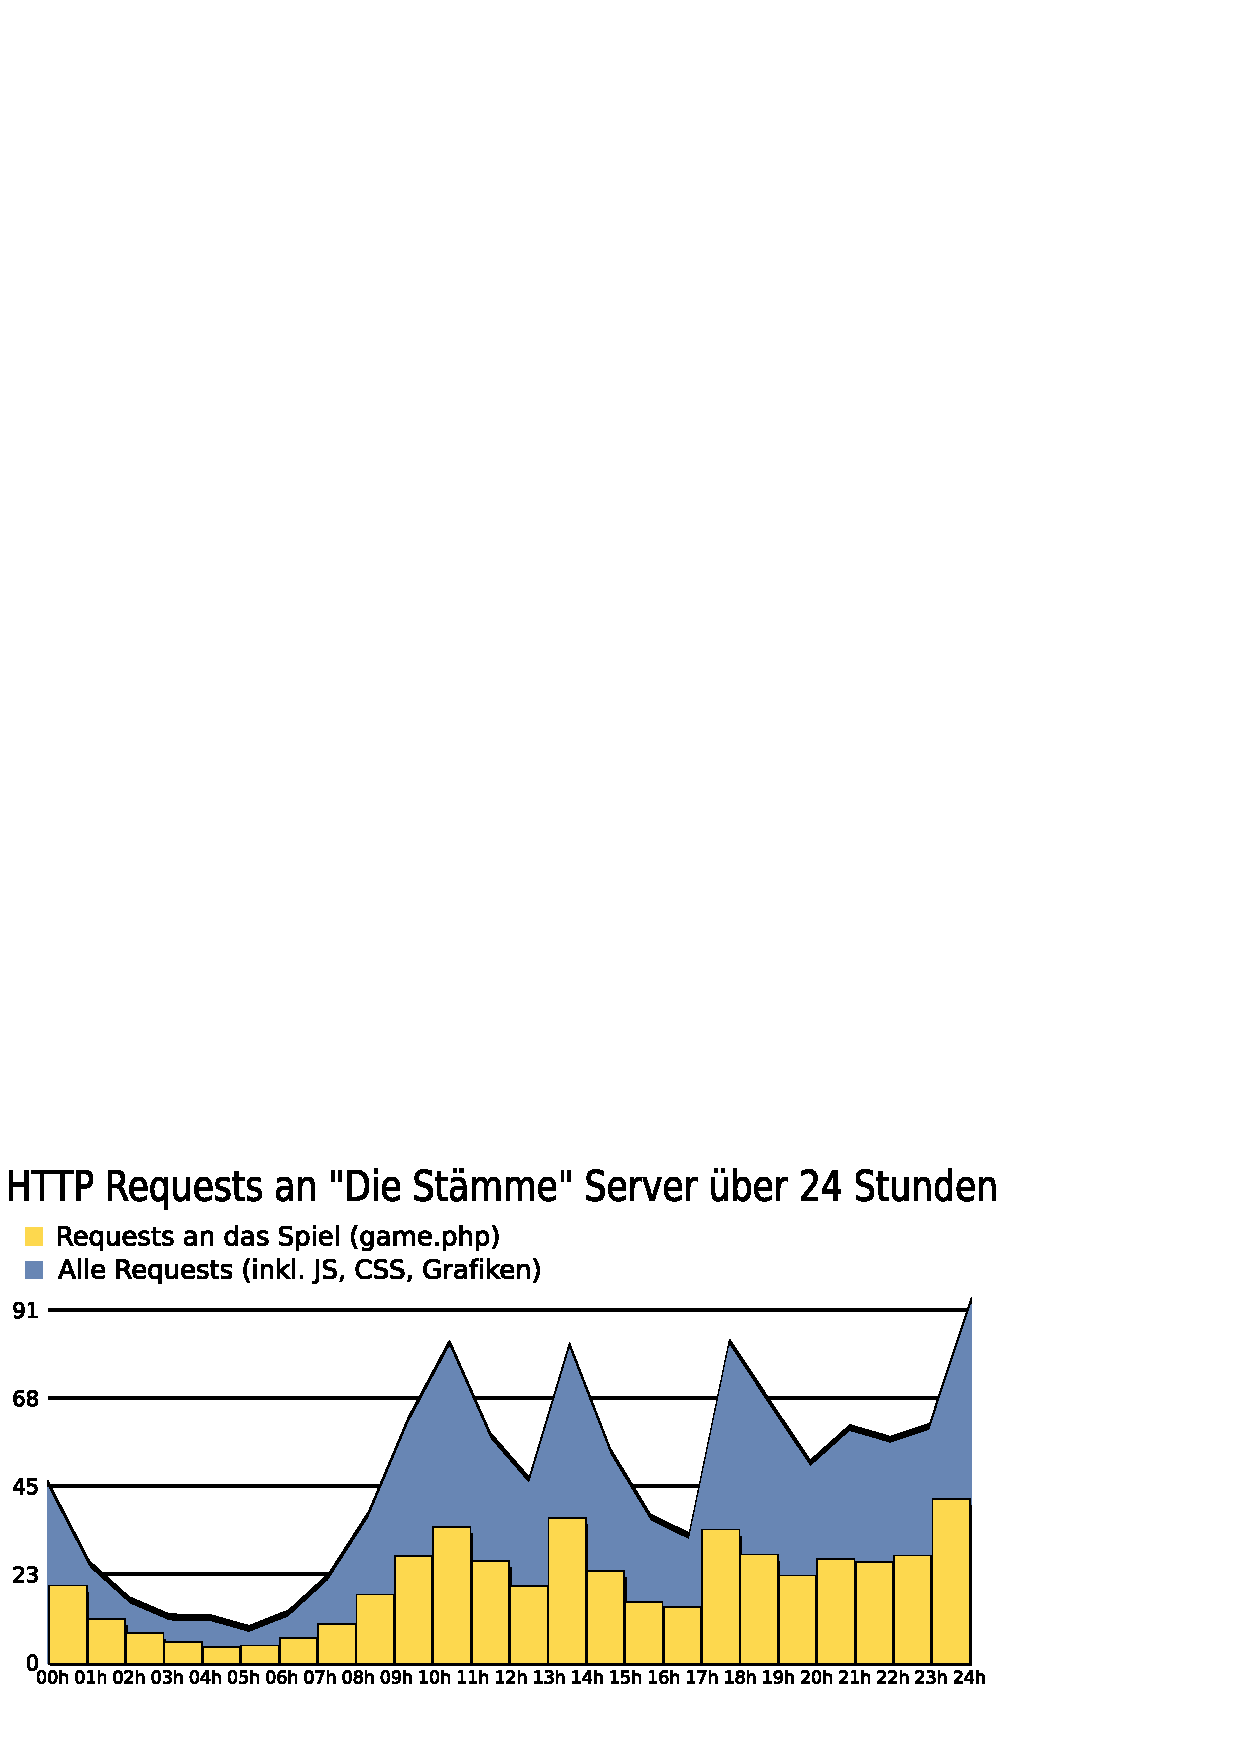
\includegraphics[height=3in]{img/requests.png}
    \caption{Verteilung der Anfragen auf 24 Stunden}
    \label{fig:requests_per_day_derivation_img}
  \end{figure}


  \subsection{Herausarbeitung von Anfragesequenzen}
  \label{subsec:request_sequences}
  Um das Lastmodell zu entwickeln ist es zunächst möglich aus den rohen Daten über die HTTP-Anfragen an den ``Die Stämme'' Server Anfragesequenzen herauszuarbeiten. Diese Sequenzen sollen Abfolgen von Aktionen eines Spielers in ihrer natürlichen Reihenfolge sein. Eine Schwierigkeit bei der Erstellung der Sequenzen ist, dass die Zugriffsdaten des Servers keine Rückschlüsse darauf zulassen, welcher Spieler eine Anfrage gestellt hat, eine Zuordnung von mehreren, nacheinander folgenden Anfragen zu einem Spieler und damit die Zusammenfassung dieser zu einer Sequenz ist daher nicht auf triviale Weise möglich. Um die Sequenzen dennoch zu erstellen wurde auf die zu jeder Anfrage gespeicherte Internetadresse des Spielers zurückgegriffen. Anfragen von einer IP werden also in einer Sequenz zusammengefasst. Die Anfragesequenzen sollen dabei nicht die Aktionen eines Spielers am gesamten Tag aneinanderreihen. Viel mehr soll eine Sequenz für die Aktionen eines Spielers bei einem Besuch des Spiels zusammenfassen. Wenn ein Spieler also mit der selben IP mehrmals pro Tag das Spiel besucht um Aktionen auszuführen sollen die Aktionen jeder dieser Besuche in jeweils eine Sequenz überführt werden. Um dies zu gewährleisten wurde sequentiell und geordnet nach Datum durch die Anfragen iteriert. Wenn eine bisher unbekannte Internetadresse gefunden wurde, wurde eine neue Sequenz erstellt die Mittels eines Hashes eindeutig und schnell zu der anfragenden IP zugeordnet werden kann. Alle folgenden Anfragen von dieser IP werden nun in diese Sequenz gespeichert. Damit nicht alle Anfragen einer IP in eine einzige,
  lange Sequenz gespeichert werden wurde mit drei verschiedenen Timeoutwerten gearbeitet. Wenn die letzte Anfrage länger 30, 60 oder 90 Minuten vor der aktuellen Anfrage gestellt wurde, wurde an dieser Stelle die alte Sequenz beendet und eine neue Sequenz begonnen. Jede Anfrage gehört also zu einer Sequenz mit 30 Minuten, einer mit 60 sowie einer mit 90 Minuten Timeout. Die Referenz zu diesen drei Sequenzen wurde jeweils in einer extra Spalte der `requests' Tabelle gespeichert um die Komplexität einer Kreuztabelle zu sparen. Da keine Erweiterung auf mehr verschiedene Timeout Werte vorgesehen ist, war dies die am schnellsten zu implementierende Lösung. Bei einer Beendung einer Sequenz rückt automatisch auch die neu eröffnete Sequenz an die Stelle der alten im Hash.

% Query zur Verteilungsanalyse der Requests per Sequenz
% select t.sub_count, count(*) from (select count(*) as sub_count from requests     where ("url" LIKE '/game.php%') and sequence_id is not null group by sequence_id) as t group by t.sub_count order by t.sub_count;

% Query zur Anzeige der Sequenzen mit bloß einem Request
% select count(*), url from requests join (select count(*) as sub_count, Min(id) as sub_id from requests group by sequence_id) as t on t.sub_id = id where t.sub_count = 1 and ("url" LIKE '/game.php%');

\subsection{URL Normalisierung}
\label{subsec:normalize_urls}
Die zu jeder Anfrage gespeicherte Ziel-URL ist für jede Anfrage sehr speziell. So wird zum Beispiel zu sehr vielen Anfragen die ID eines Dorfs in der URL kodiert, da viele Aktionen sich auf ein bestimmtes Dorf beziehen. Da diese ID und andere Parameter beinahe für jede Anfrage verschieden sind, ist es enorm schwer eine Gruppierung von Anfragen anhand der URL vorzunehmen. Zum Beispiel bei der einfachen Aktion die Übersicht über ein Dorf anzuzeigen unterscheiden sich die URLs aller Anfragen in dem Parameter ``village''. Um solch eine Gruppierung zu ermöglichen wurde eine Normalisierung der URLs vorgenommen.

Die Architektur von ``Die Stämme'' folgt einer Form des MVC Architekturmusters. Dabei wird in der URL der Controller sowie ein so genannter ``mode'' als Parameter angegeben. Der Controller wird dabei als ``screen'' bezeichet. Ähnlich wie dies in Ruby on Rails üblich ist, beinhalten Controller auch in ``Die Stämme'' meist mehrere verschiedene, mögliche Aktionen, um die der Controller eine inhaltliche Klammer darstellt. Der Parameter ``mode'' bestimmt dabei welche der Aktionen des Controllers für die aktuelle Anfrage benutzt werden soll. Anders als in Rails wird bei ``Die Stämme'' allerdings zudem zwischen einer Anzeige- und einer Ausführungsaktion unterschieden. Eine Anfrage, die den Spielzustand verändern soll gibt daher neben dem Controller (``screen'') und der Aktion zur Darstellungsvorbereitung (``mode'') auch noch die Aktion an, die die Zustandsänderung, eventuell abhängig von weiteren Parametern, herbeiführen soll. Diese Aktion wird in der URL als ``action'' bezeichnet.

Im Zuge der URL Normalisierung wurden diese drei Parameter, soweit vorhanden, aus der URL extrahiert und in separate, zur ``requests'' Tabelle hinzugefügte, Spalten an jeder Anfrage gespeichert. Dabei wurde zudem an jeder Anfrage vermerkt, ob die Anfrage bereits normalisiert wurde und, ob es eine Anfrage an die ``game.php'' ist. Die Speicherung erfolgte ebenfalls in zwei, neu hinzugefügten Spalten direkt in der ``requests'' Tabelle. Während die erste der Markierungen vor allem während des Normalisierungsprozess eine Rolle spielte, kann die zweite dazu genutzt werden noch schneller zwischen Anfragen die an die ``game.php'' und allen anderen zu unterscheiden. Da nur Anfragen an die ``game.php'' auch eine Unterteilung in ``screen'', ``mode'' und ``action'' zulassen, wurden auch nur diese Anfragen normalisiert. Alle anderen Anfragen wurden lediglich als abgearbeitet markiert. Wenn in der URL einer Anfrage zudem auch der ``village'' Parameter angegeben wurde, so wurde dieser ebenfalls zur Abfrage gespeichert. Wie beschrieben arbeitet ein Großteil der Spielaktionen mit einer Dorf ID, daher wird dieser Parameter neben den drei bereits genannten, in einer eignen Spalte in der Tabelle gespeichert. Alle anderen Parameter werden in ``JavaScript Object Notation'' (JSON) in der Spalte ``parameters'' zur Anfrage gespeichert.

Eine Übersicht über die neuen, zur Verfügung stehenden Informationen gibt Abbildung ~\ref{fig:new_requests_columns_after_url_normalization}.

  \begin{figure}[htbp]
    \centering
    \begin{tabular}{|c|c|}
      \hline
      Spaltenname & Beschreibung \\
      \hline
      screen & Controller den die Anfrage benutzt\\
      \hline
      mode & Darstellungsvorbereitungsaktion die die Anfrage benutzt\\
      \hline
      action & Spielzustandsveränderungsaktion die die Anfrage benutzt\\
      \hline
      village & ID des Dorfs auf das sich die Anfrage bezieht\\
      \hline
      parameters & Übrige, in der URL kodierte Parameter der Anfrage in JSON\\
      \hline
      url\_normalized & Boolsche Markierung, ob die Anfrage bereits von der Normalisierung erfasst wurde, oder nicht\\
      \hline
      game\_url & Boolsche Markierung, ob die Anfrage an die ``game.php'' geht, oder nicht\\
      \hline
      
    \end{tabular}
    \caption{Neue Spalten an der Tabelle ``requests'' nach der URL Normalisierung}
    
    \label{fig:new_requests_columns_after_url_normalization}
  \end{figure}
  
\subsection{Probleme bei der Arbeit mit großen Datenmengen}
\label{subsection:problems_with_large_amounts_of_data}
Bei der Analyse der Anfragedaten traten einige Probleme mit der Verarbeitung der großen Datenmenge auf, die diese Daten für 24 Stunden darstellen.

Während sich zunächst die Arbeit mit der PostgreSQL Datenbank effizient gestalte, stellten sich im Laufe der Arbeit Probleme ein, da einzelne Änderungen sehr lange dauerten. Das Problem spitzte sich bei der URL Normalisierung zu, bei der sehr viele ``UPDATE'' Operationen ausgeführt werden mussten um die Normalisierung an jeder Zeile vorzunehmen. Dieser Prozess dauerte viel länger als erwartet, was ein nicht unbekanntes Problem ist \footnote{url{http://archives.postgresql.org/pgsql-performance/2008-06/msg00117.php}, Abruf am 17. Juli 2009}. Der Grund für die langsamen ``UPDATE'' Operationen liegt im Umgang von gleichzeitigen Datenbankzugriffe von PostgreSQL. Dabei findet das so genannte ``Multiversion Concurrency Control'' (MVCC) Anwendung, ein Verfahren zur Handhabung von konkurrierenden Zugriffen auf eine Datenbank. Dabei werden von jedem Eintrag in der Datenbank verschiedene Versionen gespeichert. Innerhalb einer Transaktion sind dann stets nur die Versionen sichtbar, die vor der ersten Abfrage mittels ``SELECT'', innerhalb dieser Transaktion, bereits geschrieben wurden \footnote{Ein ausführliches Beispiel findet sich unter \url{http://www.netcraft.com.au/geoffrey/postgresql/mvcc.html}, Abruf am 17. Juli 2009}. Dieses Verfahren sorgt dafür, dass beim Aktualisieren einer Zeile ein erheblicher Mehraufwand gegenüber Datenbanksystemen besteht, die nicht das MVCC Prinzip verwenden, da eine neue Versionen der Zeile angelegt werden muss. Aus diesem Grund wurde der Versuch unternommen die Datenbank von PostgreSQL auf MySQL umzustellen. Als Speichersystem wurde dabei MyISAM eingesetzt. Damit sind zwar keine Transaktionen mehr möglich, dies ist zur Analyse der Anfragen aber auch nicht zwingend notwendig. Aufgrund der Inkompatibilität der Tabellenschemata von PostgreSQL zu MySQL, unter anderem wegen der Benutzung des Spaltentyps ``inet'', der in MySQL nicht zur Verfügung steht, wurde die Migration über den Export in ein kommasepariertes Format (CSV) vollzogen. Die Tabellen wurden aus PostgreSQL mittels:

\begin{verbatim}
  COPY requests TO '/tmp/requests.csv';
  COPY sequences TO '/tmp/sequences.csv'
\end{verbatim}

exportiert und anschließend, nachdem die beiden Tabellen manuell migriert wurden, in MySQL importiert:

\begin{verbatim}
    LOAD DATA INFILE '/tmp/requests.csv' INTO TABLE requests (id, url, ...);
    LOAD DATA INFILE '/tmp/sequences.csv' INTO TABLE sequences (id, ...);
\end{verbatim}
  
Dieser Vorgang verlief problemlos und brachte bei einer der Abfragen, die das URL Normalisierungsskript benutzte auch eine Beschleunigung um etwa den Faktor drei. Da der genau Vergleich von PostgreSQL und MySQL nicht Gegenstand dieser Arbeit ist und die dafür nötige Zeit nicht zur Verfügung stand wurden genauere Messungen nicht vorgenommen, alle genannten Zahlen und Faktoren sollen nur einen groben Überblick über die Beschleunigung geben. Bei der Analyse ist die Ausführungsgeschwindigkeit auch total irrelevant, ihre Beschleunigung diente allein dem Zweck der schnelleren Erledigung dieser Aufgabe um sich den weiteren Themen dieser Arbeit widmen zu können. 

Als sich im weiteren Verlauf der Arbeit an der URL Normalisierung herausstellte, dass das anfängliche Konzept für diese erweitert werden musste und dazu mehrmals das Tabellenschema der ``requests'' Tabelle angepasst werden musste, relativierte sich der vermeintliche Geschwindigkeitszuwachs jedoch ohnehin wieder. Dies liegt an der Art und Weise, wie MySQL die Änderungen am Tabellenschema vornimmt. Im MySQL Handbuch heißt es dazu\footnote{\url{http://dev.mysql.com/doc/refman/5.0/en/alter-table.html}, Abruf am 18. Juli 2009}:

\begin{verbatim}
In most cases, ALTER TABLE works by making a temporary copy of the original table. The alteration is performed on the copy, and then the original table is deleted and the new one is renamed.
\end{verbatim}

Es wird also die gesamte Tabelle zunächst kopiert, dann werden die Änderungen vorgenommen und dann wird die ursprüngliche Tabelle durch die neue ersetzt. Implizit bedeutet dies, dass in diesem Zuge auch alle Indizes neu berechnet werden, was bei einer solch großen Datenmenge wie in diesem Fall einen großen Zeitaufwand bedeutet. Die Änderungen an dem Tabellenschema dauerten teilweise bis zu sieben Stunden pro neuer Spalte oder neuem Index. Da bei der Ausführung des Normalisierungsskripts tatsächlich eine Zeitersparnis spürbar war, war die Rückmigration auf PostgreSQL zu diesem Zeitpunkt keine Option. Stattdessen sollte die Ausführungsgeschwindigkeit der Änderungen in MySQL optimiert werden. Dazu kamen vor allen Dingen drei MySQL Einstellungen in Frage:

\begin{itemize}
  \item Key Buffer Size
  \item Delay Key Write
  \item MyISAM Repair Threads
\end{itemize}

Die Einstellung ``key\_buffer\_size'' legt fest wie viel Arbeitsspeicher MySQL zum zwischenspeichern der Indizes verwenden kann\footnote{\url{http://dev.mysql.com/doc/refman/5.0/en/server-system-variables.html#sysvar_key_buffer_size}, Abruf am 18. Juli 2009}. Das System, das zum Auswerten der Anfragen verwendet wurde besaß 4GB Arbeitsspeicher, aber nur eine langsame Festplatte, so dass ein zu niedriger Wert hier spürbare Auswirkungen haben sollte. Nachdem der Platzbedarf aller Indizes zu diesem Zeitpunkt mittels

\begin{verbatim}
  SHOW TABLE STATUS;
\end{verbatim}

als knapp über 1 GB ermittelt wurde, wurde die ``key\_buffer\_size'' Einstellung von 250 MB auf 1,5 GB erhöht. Tests zeigten daraufhin eine deutliche Beschleunigung, auch beim Neuerstellen der Indizes.

Die Einstellung ``delay\_key\_write'' sorgt dafür, dass die Indexdaten nicht sofort auf die Festplatte geschrieben werden\footnote{\url{http://dev.mysql.com/doc/refman/5.0/en/server-system-variables.html#sysvar_delay_key_write}, Abruf am 18, Juli 2009}. Dies verhindert zwar den Zugriff von mehr als einem Datenbankserver auf die Binärdaten der Inhalte oder zum Beispiel den Einsatz des Reparaturprogramms ``myisamchk'' während der Datenbankserver in Betrieb ist, sorgt aber dafür, dass das Schreiben der Indizes wiederum deutlich beschleunigt wird. Das Umstellen dieser Eigenschaft auf den Wert ``ALL'', zur globalen Nutzung der Funktion beschleunigte das Ändern der Tabellenschemata erneut.

Als Letzter Ansatzpunkt zur Optimierung des Verhaltens beim Ändern der Tabellen wurde die Einstellung ``myisam\_repair\_threads'' betrachtet, die die Anzahl der Threads einstellen lässt, mit der in MyISAM Tabellen eine Neuindizierung stattfindet\footnote{\url{http://dev.mysql.com/doc/refman/5.1/en/server-system-variables.html#sysvar_myisam_repair_threads}, Abruf am 18. Juli 2009}. Da das Auswertungssystem über zwei CPU Kerne verfügte und die Tabelle über mehr als einen Index, wäre durch die Nutzung von zwei Threads hier ebenfalls ein deutlicher Geschwindigkeitszuwachs zu erwarten. Das Umstellen des Wertes von ``1'' auf ``2'' brachte allerdings keine Veränderung. Auch war nach der Umstellung weiterhin nur ein Kern bei der Neuindizierung ausgelastet.

Nach diesen Verbesserungen brauchte der Prozess der Normalisierung aber immer noch sehr lange, so dass entschieden wurde diesen genauer zu untersuchen.

Der Prozess lief zu diesem Zeitpunkt in etwa wie folgt ab:

\begin{verbatim}
  Hole das Datum der ersten Anfrage, sortiert nach dem Datum
  Berechne das Startdatum als mitternacht(obiges Datum + 1 Tag)
  Hole 10.000 Zeilen, die noch nicht normalisiert wurde, beginnend ab dem\  
    Startdatum, sortiert nach dem Datum
  Solange dies Zeilen zurückliefert
    Für jede Zeile
      Normalisiere URL und markiere diese als normalisiert 
    EndeFür
  EndeSolange
\end{verbatim}

Eine Analyse ergab, dass der größte Teil der Zeit für diesen Algorithmus nicht die Änderungen an den Zeilen ausmachten, sondern die Abfrage der Zeilen. Für diese wurde folgende SQL Query verwendet:

\begin{verbatim}
  SELECT * FROM `requests` WHERE `url_normalized` = false AND \
    `date` >= '2009-06-07 00:00:00' AND date < '2009-06-08 00:00:00' \
    ORDER BY DATE LIMIT 10000;
\end{verbatim}

Die Überprüfung dieser Abfrage mittels ``EXPLAIN'' lieferte schnell den Grund für deren langsame Ausführung: Die Tabelle ``requests'' besaß zwar einen Index auf der Spalte ``url\_normalized'' sowie auf der Spalte ``date'', ein Index über beide Spalten war aber nicht vorhanden, so dass MySQL standardmäßig auf den Index über der ``url\_normalized'' Spalte zurückgriff. Ein forcieren der Nutzung des Datumsindex brachte schon eine Verdopplung der Ausführunsgeschwindigkeit, war aber im Normalisierungsskript schwer umzusetzen, da dieses eine Objektrelationale Abbildung mittels ``Sequel''\footnote{\url{http://sequel.rubyforge.org/}, Abruf am 23. Juli 2009} benutzte, mit der ein Forcieren eines Index nicht möglich ist. Zwar lässt ``Sequel'' die Verwendung von handgeschriebenen Abfragen zu, dies hätte allerdings viel von dem Komfort des Einsatzes einer solchen Lösung zerstört, es wurde daher nicht darauf zurückgegriffen. Stattdessen wurde der eigentliche Algorithmus so modifiziert, dass er keinen Gebrauch mehr von der ``url\_normalized'' Spalte machte und damit nur noch den Datumsindex benötigte.

Der Algorithmus funktionierte nun wie folgt:
\begin{verbatim}
  Hole das Datum der ersten Anfrage, sortiert nach dem Datum
  Berechne das Startdatum als mitternacht(obiges Datum + 1 Tag)
  Hole 10.000 Zeilen, beginnend ab dem Startdatum, sortiert nach dem Datum
  Solange dies Zeilen zurückliefert
    Für jede Zeile
      Normalisiere URL und markiere diese als normalisiert 
    EndeFür
    Setze Startdatum auf Datum der letzten, geholten Zeile 
  EndeSolange
\end{verbatim}

Mit diesen Änderungen konnte dann die URL Normalisierung innerhalb weniger Stunden ausgeführt werden.

Nach der Normalisierung verbesserte sich die Situation erneut. Durch die zur Verfügungstellung eines dedizierter Hardware als Datenbankserver für die Analysen konnten die gemessenen Anfragen um mehr als den Faktor 60 beschleunigt werden. Zum Beispiel benötigte die folgende Anfrage:

\begin{verbatim}
   SELECT COUNT(*) FROM `requests` WHERE `date` <= '2009-06-07 14:00:00' AND \
    `url_normalized` = true;
\end{verbatim}

auf der ursprünglich zur Analyse verwendeten Hardware 3 Minuten und 5 Sekunden, während sie auf dem dedizierten Datenbankserver in 2,84 Sekunden abgearbeitet wurde.


% Sequenzwiederherstellung
% INSERT INTO sequences (id, type) SELECT DISTINCT requests.short_timeout_sequence_id, 1 FROM requests;
% INSERT INTO sequences (id, type) SELECT DISTINCT requests.medium_timeout_sequence_id, 1 FROM requests;
% INSERT INTO sequences (id, type) SELECT DISTINCT requests.long_timeout_sequence_id, 1 FROM requests;
% Manchmal komische DUPLICATE ENTRY Fehler aber so what, irgendwann funktionierte es.

%  ec2 pfad
% /home/webuser/helloworld/logs
% Image: http://alestic.com which are pretty popular for production use.
% Setup: apt-get update && apt-get upgrade -y && apt-get install -y apache2


  \section{Lastsimulation}
  Aus den gewonnenen Erkenntnissen aus der Lastanalyse wurde ein System zum Generieren von Lastmodellen entwickelt, dass den Charakteristika der analysierten, echten Last möglichst nahe kommt. Dabei musste aber sichergestellt werden, dass auch eine gezieltes Abweichen vom echten Vorbild möglich ist um so beispielsweise Funktionen, die in ``Die Stämme'' enthalten sind, nicht aber im im Rahmen dieser Arbeit entwickelten Spiel, herauszufiltern.
  %TODO: Warum nicht echte Daten? Könnte man ja auch filtern
  
  Nach der Generierung eines Modells müssen auf Grundlage dessen die HTTP Anfragen an das Spiel generiert werden um sein Verhalten unter der Last zu überprüfen. Dazu wurde ein Verfahren entwickelt, dass dies einfach ermöglicht.
  
  \subsection{Lastmodell}
  Das Lastmodell soll die Abläufe, die ein Spieler im Spiel tätigt möglichst realistisch wiedergeben, aber gleichzeitig dazu in der Lage sein verschiedene Lastverläufe, also Sequenzen von Benutzeraktionen zu generieren. Aus den Anfragesequenzen, die während der Lastanalyse herausgearbeitet werden müssen daher Aktionsfolgen extrahiert werden. Diese Aufgabe erinnert stark an die Textgenerierung, bei der aus vorgegebenen, echten Texten synthetische erzeugt werden sollen. Zu diesem Zweck werden häufig Markovketten verwendet.
  % TODO: Literaturverweis Markov zur Textgenerierung?
  Markovketten nutzen dabei die Annahme, dass jeder Zustand einer Folge abhängig von seinen direkten $n$ Vorgängern ist. Explizit bedeutet dies, dass ein Zustand   $s_i$ einzig abhängig ist von den Zuständen $s_{i-n...i-1}$. Für die Lastmodellierung im Rahmen dieser Arbeit bietet sich ein solches Modell ebenfalls an. Bei Betrachtung des Spielaufbaus von ``Die Stämme'' ist davon auszugehen, dass die allermeisten Aktionen der Spieler abhängig von wenigen ihrer vorangehenden Aktionen sind. Natürlich ist es im Spiel für den Erfolg der Spieler wichtig, dass diese eine Strategie verfolgen, die mitunter sehr komplexe Ausmaße annehmen kann. Die einzelnen Teile jeder Strategie lassen sich aber in kurze Ketten von Handlungen herunterbrechen. Wenn ein Spieler beispielsweise ein Gebäude in einem Dorf bauen will, so ist eine wahrscheinliche Handlungskette folgende:
  
  \begin{enumerate}
    \item Aufrufen der Dorfübersicht
    \item Aufrufen des Hauptgebäudes
    \item Abschicken des Bauauftrages
  \end{enumerate}
  
  Auch wenn also das Spiel erfordert in komplizierten Strategien zu denken, so ist es für die Lastsimulation vollkommen unerheblich, da es die Auslastung des Spiels nicht beeinflusst ob ein Spieler mit besonderer Finesse verschiedene Aktionen hintereinander reiht. Wichtig bleibt aber, dass die Aktionen selbst in korrekter Weise generiert werden können. 
  % TODO: Warum?
  Eine Markovkette eignet sich daher gut als Basis für ein solches Lastmodell. 
  
  \subsubsection{Markovkette}
  Die für das Lastmodell verwendete Markovkette ist zweistufig. Jede Anfrage hängt also von den vorhergehenden zwei Anfragen ab. Die Verwendung von höher stufigen Ketten würde die Gefahr einer Überanpassung bergen, bei der die Kette lediglich noch Abfolgen reproduzieren würde, die genau so auch in der analysierten Last vorkommen. Eine Markovkette ersten Grades würde dagegen die Zusammenhänge von Anfragen im Spiel nicht ausreichend abbilden. Natürlich sind im Spiel nicht alle Aktionen ,wie im oben gezeigten Beispiel, auch drei Schritte lang. Die Grundannahme von dreischrittigen Aktionen und daher die Verwendung einer zweistufigen Markovkette ist ein guter Kompromiss zwischen der Überanpassung und der völligen Ungebundenheit bei der Entscheidung für die nächste Anfrage.
  % TODO: Literatur Überanpassung/overfitting?
  
  \paragraph{Implementierung}
  \label{par:markov_implementation}
  Die verwendete Markovkette basiert auf einem Baum der Tiefe drei. Auf der obersten Ebene stehen dabei alle Zustände denen mindestens noch zwei weitere folgten. Jedes dieser Blätter hat wiederum alle Zustände die auf ihn selbst folgten als Blätter. Und diese wiederum alle Zustände die auf diese folgten. An den Blättern der untersten Ebene ist notiert wie oft genau dieser Pfad, von der Wurzel bis zu ihnen, vorkam. Für die Sequenz:
  
  \begin{verbatim}
    a,b,d,b,a,b,a,c,b,a,c
  \end{verbatim}
  
  sieht der Baum dann wie folgt aus:
  
  \begin{verbatim}
         a        b        c   d
        / \      / \       |   |
      b    c    d   a      b   b
     / \   |    |  / \     |   |
    d   a  b    b b   c    a   a
    1   1  1    1 1   2    1   1
  \end{verbatim}
  
  So ist es leicht zu bestimmen was für eine gegebene Folge von 2 Zuständen die Wahrscheinlichkeiten aller Folgezustände ist. Auf \verb|b,a| folgt in $\frac{2}{3}$ der Fälle ein \verb|c| und in $\frac{1}{3}$ der Fälle ein \verb|b|. Auch wenn weniger als zwei Zustände gegeben sind lassen sich die Wahrscheinlichkeiten der Folgezustände einfach errechnen indem man die Summe aller möglichen Folgepfade errechnet und dabei lediglich das erste Element dieser Folgepfade betrachtet. Auf ein \verb|b| folgt beispielsweise entweder die Folge \verb|d,b| (Wahrscheinlichkeit $\frac{1}{4}$), \verb|a,b| (Wahrscheinlichkeit $\frac{1}{4}$) oder \verb|a,c| (Wahrscheinlichkeit $\frac{2}{4}$). Da aber nur der auf das \verb|b| folgende Zustand interessiert kann man die Schlussfolgerung gezogen werden, dass auf \verb|b| mit einer Wahrscheinlichkeit von $\frac{1}{4}$ ein \verb|d| folgt und mit $\frac{3}{4}$ ein \verb|a|.
  
  Diese Implementierung erlaubt auch ein einfaches ``lernen'' von neuen Folgen.
  Dazu wird lediglich über alle dreistelligen Folgen in der zu lernenden Folge iteriert und der Baum wird mit diesen Unterfolgen aktualisiert. Bei bereist existierenden Pfaden muss dazu lediglich der Zähler am untersten Blatt inkrementiert werden, Pfaden die im Baum noch nicht vorhanden sind werden diese an die passende Stelle eingehangen und der Zähler wird auf 1 initialisert.
  
  \paragraph{Erstellung}
  \label{par:markov_generate}
  Für jeden Typ von Anfragesequenz (Timeout von 30, 60 oder 90 Minuten siehe \ref{subsec:request_sequences}) musste eine eigene Markovkette erstellt werden. Dazu wurde zu Beginn der beschriebene Baum erstellt und dann nach und nach jede Sequenz aus der Datenbank abgefragt und in den Baum eingespeist. Dabei wurde an das Ende einer Sequenz stets ein Endsymbol angehängt. Dies dient dazu um auch Wahrscheinlichkeiten für das Enden einer Sequenz nach einer bestimmten Folge aufstellen zu können. Um die Markovkette speichern zu können wurde diese am Ende direkt als Ruby Datenstruktur in ein Binärformat überführt \footnote{\url{http://www.ruby-doc.org/core/classes/Marshal.html}} und in eine Datei geschrieben.
  
  \paragraph{Kodierung der Anfragen}
  \label{para:request_encoding}
  Um Anfragen in die Markovkette einzutragen wurde auf die URL Normalisierung der Anfragen (siehe \ref{subsec:normalize_urls}) zurückgegriffen und lediglich die Parameter ``Screen'', ``Mode'', ``Action'' und die HTTP Methode in der Kette gespeichert. Lediglich durch diese Generalisierung von Anfragen war es überhaupt Anfragen auf ihre Gleichheit zu überprüfen und damit auch eine sinnvolle Markovkette aufzubauen. Anderenfalls bestünde die Kette aus $1,7$ Millionen einzigartigen Pfaden.
  
  Um die Datenstruktur der Markovkette schlank zu halten wurde der Fakt ausgenutzt, dass es eine endliche Anzahl von verschiedenen Belegungen für jeden der in der Kette gespeicherten Parameter gibt. Es gibt sogar für keinen der Parameter mehr als $2^8$ verschiedene Belegungen. Daher konnten die 4 Parameter in Form von 4 Byte und einer Zuordnungstabelle von Bytewert zu Belegung des Parameters gespeichert werden.
  
  Bei dieser Art der Kodierung gehen allerdings alle weiteren Parameter der Anfragen verloren. Dieser Umstand ist allerdings kein Problem, da die Parameter später keine Rolle spielen werden. Um bei der Lastgenerierung nicht auch im Kontext der aktuellen Anfrage stimmige Parameter für die Spielaktion zu erzeugen, die die Anfrage auslösen soll werden diese einfach vollständig weggelassen. Auf Seiten des Spiels werden die notwendigen Parameter dann zufällig gewählt. Ein solches Vorgehen ist möglich, da es im Rahmen dieser Arbeit nicht um die Simulation eines sinnvollen Spielgeschehens sondern ausschließlich um eine Lastanalyse des entwickelten Spiels geht. Das genaue Vorgehen beim zufälligen Wählen aller Parameter ist unter \ref{sec:game_dev_random_params} zu beschrieben.
  
  % TODO: Beschreibung der zufälligen Parameterwahl im Zuge der Spielentwicklung beschreiben und Ref klarbekommen
  
  \subsection{Lastgenerierung}
  Um auf Grundlage des Lastmodells auch HTTP Anfragen abschicken zu können bedarf es noch einiger weiterer Schritte.
  
  \subsubsection{Sequenzgenerierung}
  Zunächst wurden aus den Markovketten konkrete Sequenzensammlungen erstellt. Im Rahmen dieser Arbeit wurde je zwei Sequenzsammlungen zu den Markovketten erstellt, die auf den Anfragesequenzen mit 60 minütigem Timeout erstellt und je eine Sequenzsammlung zu den beiden anderen Markovketten zu den Anfragesequenzen mit 30 und 90 minütigem Timeout. Jeder der Sammlungen umfasst 30.000 Sequenzen und wurde, genau wie die Markovketten, nach ihrer Erstellung im Binärformat gespeichert.
  
  Die Generierung von Sequenzsammlungen aus den Markovketten ist trivial. Beginnend mit einer leeren Sequenz wurden die Nachfolgerwahrscheinlichkeiten für die letzten zwei Elemente der Sequenz an der Markovkette abgefragt und dann aus den Nachfolgern, gewichtet nach deren Wahrscheinlichkeit der Nachfolge, zufällig einer ausgewählt. Wie beschrieben (siehe \ref{par:markov_implementation}) ist dies problemlos auch mit leeren oder nur ein Element umfassenden Sequenzen möglich. Sobald mittels dieses Prozesses das Endsymbol (siehe \ref{par:markov_generate}) erreicht wurde, wurde die Sequenz zur Sequenzsammlung hinzugefügt und eine neue, leere Sequenz begonnen.
  
  Die Generierung wurde zudem auf acht Prozesse aufgespalten. Da diese auf dem gleichen System vorgenommen wurde wie auch der letzte Teil der Lastanalyse konnten damit alle acht Prozessorkerne ausgenutzt und der Prozess so beschleunigt werden.
  
  % TODO: Diagram einbauen: Sequenzlängen
  
  \subsubsection{Werkzeug zur Lastsimulation}
  Die generierten Sequenzen müssen nun in HTTP Anfragen umgesetzt werden. Da eine ganze Reihe von Werkzeugen zur HTTP Lastsimulation existieren lag der Fokus in diesem Bereich auf der Untersuchung dieser bestehenden Lösungen und ihrer Eignung im Rahmen dieser Arbeit.
  
  Neben den beiden bekannten, älteren Programmen ``Apache Bench'' und ``httperf'' wurde zudem das relativ neue ``Faban'' getestet. 
  
  %TODO Erklären wieso nur diese drei.
  
  \paragraph{Faban}  ~\\
  \url{http://faban.sunsource.net/}
  \\
  ~\\
  Eine Java Benchmark Lösung mit der es, anders als mit einfachen Tools wie
  beispielsweise AB oder httperf, möglich sein soll auch komplexere Benchmarks
  durchzuführen. Die Benchmarks werden dabei nicht konfiguriert sondern können
  in Java programmiert werden. Faban sorgt dann mit einer Infrastruktur aus 
  einem ``Master Server'' und beliebig vielen, auch auf anderen Hosts als der
  Master Server liegenden, Agenten dafür, dass dieser Benchmark aufgeführt und
  die Ergebnisse der einzelnen Agenten wieder zusammengeführt werden.
  
  Die Konfiguration und Benutzung von Faban gestaltet sich schwierig. Nachdem 
  dann auch aus der Dokumentation hervorgeht, dass die Implementierung von
  zu verfolgenden Klickpfaden per Markovketten ein Erweitern des Faban Systems
  unumgänglich machen wird das Simulieren von Lasten mit Faban zunächst zu 
  Gunsten der Evaluierung anderer Systeme aufgegeben.
  
  \paragraph{Apache Bench - ab}  ~\\
  \url{http://httpd.apache.org/docs/2.0/programs/ab.html} 
  \\
  ~\\
  Apache Bench (\textit{ab}) ist ein Kommandozeilen Programm, dass es auf einfache Weise
  erlaubt einen Benchmark auf eine einzelne Ressource per HTTP durchzuführen.
  \textit{ab} misst dabei vor allem die Auslieferungszeit der Ressource und errechnet
  einige Hilfswerte wie zum Beispiel die bedienten Anfragen pro Sekunde.
  Auch wenn \textit{ab} die vorgestellte Aufgabe gut erfüllt eignet es sich nur sehr
  eingeschränkt für das Testen einer Folge von Ressourcen, wie es im Lastmodell
  dieser Arbeit vorgesehen ist. Der einzige Weg mit \textit{ab} solche Folgen 
  abzuarbeiten wäre es für jede Ressource einen neuen \textit{ab} Prozess zu starten, was
  untereinander zu Problemen bei der Synchronisierung führen würde, 
  schwer zu kontrollieren wäre und zudem den Nachteil hätte, dass die Ergebnisse
  schwer zusammenführen sind.
  
  Aus diesen Gründen wird vom Gebrauch von \textit{ab} als Lastsimulator für diese Arbeit
  abgesehen.
  
  \paragraph{httperf}  ~\\
  \url{http://www.hpl.hp.com/research/linux/httperf/}
  \\
  ~\\
  httperf ist, ähnlich wie \textit{ab}, ein Kommandozweilen Werkzeug zum
  Durchführen von Benchmarks per HTTP. Auch die dabei gemessenen Werte ähneln
  denen von \textit{ab}. Im Gegensatz zu \textit{ab} erlaubt httperf allerdings
  nicht nur das Benchmarken einer einzelnen Ressource, sondern auch das einer
  ganzen Folge von Ressourcen. Die Konfiguration dieser Folgen ist sehr 
  detailliert möglich so sind insbesondere auch Wartezeiten zwischen zwei 
  Aufrufen und das Gleichzeitige Aufrufen mehrerer Ressourcen zu einem Zeitpunkt
  möglich, um so beispielsweise den Aufruf eines HTML Dokuments sowie aller
  darin referenzierten JavaScript-, Bild- und Cascading Style Sheets (CSS)-Dateien zu simulieren. Diese Folgen sind allerdings auf 1000 pro httperf Prozess begrenzt. Für eine Verwendung von httperf müssten also auf jeden Fall, pro ausführendem Rechner mehrere httperf Prozesse gestartet werden. Zudem ist die Konfiguration von httperf nicht trivial, da einige Parameter änliche Verhaltensweisen steuern und es so erst nach sehr vielen Versuchen möglich war httperf mit einer gegebenen Folge zu starten aus der es verschiedene, einzelne Sequenzen der Folge mit parallelen Verbindungen zum Webserver abgearbeitet hat. Selbst dann war zum Beispiel das Einstellen der Anzahl der gleichzeitig benutzten Verbindungen nicht trivial.
  
  \paragraph{Eigene Lösung}
  ~\\
  ~\\
  \label{para:load_generator_custom_solution}
    Aufgrund dieser Unzulänglichkeiten der bestehenden Lösungen wurde sich dazu entschlossen eine eigene, triviale Lösung für das Problem zu entwerfen. Da der gesamte Testverlauf anhand der Anfragenaufzeichnungen des Webservers getestet werden kann, kann der Lastgenerator trivial gehalten werden. Er muss lediglich das absetzen von HTTP Anfragen an einen Webserver an eine vorgegebene Reihe von Ressourcen erlauben und dabei möglichst mehrere Verbindungen zu einem Server gleichzeitig benutzen können. Da mit dem Arbeitsrechnerpool der Universität Bremen ein großer Bestand an verwendbaren Rechnern zum Ausführen des Lastgenerators besteht muss dieser auch nicht in seiner Ausführungsgeschwindigkeit optimiert werden, da die Vielzahl an gleichzeitig verwendeten Rechnern etwaige Unzulänglichkeiten hier wieder wett macht.
    
    Der Lastgenerator besteht aus zwei wesentlichen Teilen. Der erste bekommt als Eingabe für $n$ Benutzer je eine Reihe von Sequenzen welche wiederum eine Reihe von Anfragen enthalten. Die Abarbeitung geschieht für alle Benutzer parallel, indem das Programm per \verb|fork| $n$ Kindprozesse erstellt, die die eigentliche Arbeit leisten. Diese stellen nun der Reihe nach alle Anfragen aus allen Sequenzen des Benutzers für den sie zuständig sind an den Server.
    
    Der zweite Teil sorgt dafür, dass der Lastgenerator verteilt im Arbeitsrechnerpool der Universität ausgeführt werden kann. Dazu werden die Rechner angegeben, die als Lastgeneratoren dienen sollen. Auf diesen werden dann zunächst der Lastgenerator selbst, sowie die vom jeweiligen Rechner abzuarbeitenden, generierten Sequenzen übertragen. Im zweiten Schritt wird dann der Lastgenerator auf den Rechnern gestartet. Dies geschieht per SSH, bzw. SCP.
    
  \subsection{Sequenzübersetzung}
  Um keine zu starke Bindung an den Lastgenerator einzugehen sollen die in einer Sequenzsammlung generierten Anfragen, die zu diesem Zeitpunkt einzig aus dem Ziel der Anfrage in der beschriebenen 4-Byte-Kodierung (siehe \ref{para:request_encoding}) vorliegen, in einem Schritt vor der Lastgenerierung zu URLs der anzufragenden Ressourcen übersetzt werden.
  
  Um aus einer Sequenzsammlung korrekte Eingabedaten für den Lastgenerator zu erstellen müssen die Sequenzen der Sammlung zunächst aufgeteilt werden. Bei $n$ Instanzen des Lastgenerators und $m$ zu simulierenden, gleichzeitigen Benutzern auf dem System und $k$ Sequenzen in der Sequenzsammlung geschieht die Aufteilung wie folgt:
  
  Es werden $n$ Eingaben erstellt mit je $\frac{m}{n}$ Benutzern die jeweils $\frac{k}{n}$ Sequenzen abarbeiten. Da jede Sequenz unterschiedlich lang ist, sind die Abfolgen der einzelnen Benutzer dennoch nicht zu uniform.
  
  Da auch der Lastgenerator in Ruby geschrieben ist kann die Eingabe erneut per Marshalling direkt als Datenstruktur gespeichert werden.
  
  Folgende Probleme sind weiterhin zu lösen:
  
  \begin{enumerate}
    \item Übersetzung des Tupels ``Screen'', ``Mode'', ``Action'' in eine URL
    \item Filterung von Anfragen die im neu geschriebenen Spiel nicht vorkommen
  \end{enumerate}
  
  Die Übersetzung in eine vollständige HTTP Anfrage kann generell nur unzureichend geschehen, da keinerlei Parameter zu der kodierten Aktion mehr vorhanden sind. Löst die Aktion beispielsweise den Bau eines Gebäudes im Spiel aus, so muss natürlich in der Anfrage auch übergeben werden welches Gebäude gebaut werden soll. Für die Lastsimulation sind diese Parameter allerdings unerheblich. Sie werden an dieser Stelle weggelassen und später vom entwickelten Spiel zufällig gewählt (siehe \ref{sec:game_dev_random_params}). Es geht also ausschließlich darum wie ``Screen'', ``Mode'' und ``Action'' zu einer URL überführt werden können. Dieser Vorgang wird in Ruby modelliert, so dass sowohl eine einfache Zuordnungstabelle eingesetzt werden kann, als auch komplizierterer Mechanismen, die programmiert werden.
  % TODO: wie wurde das letztendlich erledigt?!
  % TODO: Wie genau ändert sich was? Ref zur Spielkonzeption?
  
  Das Filtern von Anfragen ist ein wichtiger Schritt, da das entwickelte Spiel aus Zeitgründen keine vollständige Kopie von ``Die Stämme'' sein kann. Einige, gar nicht im neuen Spiel vorhandene Teile müssen also herausgefiltert werden. Der Grund für eine solch späte Filterung zum Beispiel gegenüber eines Herausfilterns der entsprechenden Anfragen schon bei der Erstellung der Markovkette liegt in der einfachen Anpassungsfähigkeit begründet. Der ganze Vorgang der Aufteilung der Sequenzsammlung in korrekte Eingabedaten für den Lastgenerator dauert nur wenige Sekunden. Sobald sich also am entwickelten Spiel etwas ändert, dass eine Änderung am Filterprozess notwendig macht kann dies ohne großen Aufwand realisiert werden. Das Erstellen der Markovkette dagegen dauert deutlich länger. Das späte Filtern bedeutet also einen großen Zugewinn an Flexibilität.
  
  Auch das Filtern wird in Ruby modelliert was auch hier ein triviales Aussortieren, beispielsweise mit einer Filterliste, möglich aber gleichzeitig auch kompliziertere Filterkriterien anwendbar macht.
  
  \subsection{Verteilung der Prozesse}
  Um eine realistische Lastsimulation durchführen zu können darf die Last nicht von einem einzelnen Rechner aus generiert werden. Auf den echten ``Stämme'' Welten befinden sich, je nach Definition, bis zu 1000 Spieler gleichzeitig und stellen Anfragen an den Server. Dies von einem einzelnen Rechner aus zu simulieren kann zum einen zu Bandbreitenproblemen auf Seiten des generierenden Systems führen und zum anderen kann das generierenden System unter Umständen nicht die benötigte Leistung bereitstellen um ausreichend Last zu generieren.
  % TODO: Warum sind viele Rechner noch gut?
  Die Verteilung auf verschiedene Rechner ist bei dem vorgestellten Lastgenerator von Anfang an vorgesehen (siehe \ref{para:load_generator_custom_solution}).
  
  
  \subsection{Testausführung}
  Zur Ausführung der Lasttests dienen zehn Arbeitsplatzrechner des Fachbereichs Informatik der Universität Bremen als Last generierende Systeme. Diese sind in der Universität mit ausreichender Bandbreite an der Internet angeschlossen. Die Tests wurden zudem zwischen 00 und 6 Uhr durchgeführt, in dieser Zeit ist kein physischer Zugang zu den Arbeitsplatzrechner möglich, da das Gebäude abgeriegelt ist. Auch konnte mittels Stichproben keine nennenswerte Aktivität an den Systemen durch Fernzugriffe mittels SSH festgestellt werden.
  
  Der Lasttest selbst wird durch ein Ruby Programm koordiniert, dass per SSH den Test vorbereitet und ausführt.
  
  \subsection{Validierung des Vorgehens}
  Um zu Überprüfen ob das beschriebene Vorgehen auch die für diese Arbeit geforderten Charakteristika aufweist wurde die Lastgenerierung an einem Beispiel getestet. Dabei wurde nicht der Webserver betrachtet sondern die testenden Systeme.
  
  Auf der Serverseite kam dabei ein Apache Webserver zum Einsatz, der lediglich eine einzige, etwa 2 Kilobyte große Datei für alle Anfragen auslieferte. Dazu wurde die Apache Erweiterung ``mod\_rewrite'' so eingerichtet, dass die Anfrage auf jede Ressource in eine Anfrage auf die Datei \verb|index.html| umgedeutet wurde, an die dann per GET Parameter ``Screen'', ``Action'' und ``Mode'' notiert wurden. Zu Beginn des Tests wurde die Anfragenaufzeichnung des Webservers zurückgesetzt, so dass sich nach dem Test einzig die Anfragen des Tests in der Aufzeichnung befinden.
  
  Zur Lastgenerierung wurde eine Sequenzsammlung aus $30.000$ Sequenzen benutzt, die wiederum aus der Markovkette der Anfragen mit einem Timeout von 60 Minuten erzeugt wurde. Die Sequenzen wurden auf $10$ Arbeitsplatzrechner im Universitätsnetz ausgeführt und insgesamt $1.000$ gleichzeitige, simulierte Benutzer verteilt.
  
  Der Test stellte knapp über zwei Millionen Anfragen an einen Webserver, der nicht im Universitätsnetz angebunden war, die Anfragen mussten also tatsächlich über das Internet gestellt werden. Die Ausführung dauerte $TODO: XXX$ Sekunden. Eine Analyse der Anfragenaufzeichnung auf dem Webserver ergab die folgende Verteilung von Anfragen nach anfragenden Rechnern:
  
  % TODO: Diagramm aus test access.log nach IP gruppiert
  
  Zudem wurden die Anfragen nach Minuten gruppiert und jeweils der Schnitt der erreichten Anfragen pro Sekunde ermittelt:
  
  % TODO: Grafik der Req/Sek.
  
  Der Lastgenerator arbeitet also auf den Arbeitsplatzrechnern wie erwartet verteilt, und kann deutlich mehr Anfragen pro Sekunde erzeugen als benötigt. Während des Tests wurden dabei mehr als $2.000 \frac{Anfragen}{Sekunde}$ erzielt. Dieser Tests gibt natürlich keinen Aufschluss über die Kapazität des Webservers, sondern lediglich über das zur Lasterzeugung eingesetzten System. Dabei kann dessen Leistung eventuell durch externe Faktoren wie zum Beispiel den Webserver oder die Internetanbindung der Universität oder des Webservers begrenzt werden, die gezeigte Leistung liegt aber bereits um etwa den Faktor 20 über dem, was das neu programmierte Spiel liefern soll. Bei diesem wird eine Leistung von 100 Anfragen pro Sekunde angestrebt.
    
  \section{Anwendungsentwicklung}
  \subsection{Konzeption}
  Das neu zu programmierende Spiel soll dem Spiel ``Die Stämme'' möglichst nahe kommen um eine hohe Vergleichbarkeit der beiden Spiele zu erreichen. Zunächst sollen daher die grundlegenden Mechanismen des Vorbilds erläutert werden, bevor beschrieben wird wie der enorme Umfang von diesem auf ein Maß reduziert werden kann, so dass eine Kopie im Rahmen dieser Arbeit möglich ist.
  
  Daran schließt sich ein genaues Konzept des neu zu programmierenden Spiels an.
  
  \subsubsection{Die Stämme - Das Spielprinzip}
  \referencedquote
  {
    Die Stämme (kurz: ``DS'') ist ein 2003 von der Firma InnoGames GmbH gestartetes Browserspiel, das sich um die Eroberung von feindlichen Dörfern im Mittelalter dreht\ldots
    Es existiert kein offizielles Spielziel, jedoch wird der Erfolg meist in einer hohen Anzahl von Punkten gesehen. In der virtuellen Welt startet jeder Spieler mit einem Dorf, dessen Ausbau erforderlich ist, um neue Gebäude - und damit auch verbesserte Einheiten - erschaffen zu können. Sehr bald schon rücken kriegerische Auseinandersetzungen in den Mittelpunkt des Spiels: Es gilt Dörfer anderer Spieler zu erobern und die eigenen zu schützen. Dazu müssen Truppen rekrutiert werden,\ldots . Die Kämpfe selbst werden nicht dargestellt; die Spieler erfahren in Berichten nur deren Ausgang. Um das Teamplay zu fördern, können sich Spieler in Gruppen - im Spiel Stämme genannt - zusammenschließen und sich so gegenseitig mit Ressourcen und Truppen unterstützen.
  }
  {
    Wikipedia\footnote{
 \url{http://de.wikipedia.org/w/index.php?title=Die_St\%C3\%A4mme&oldid=63674653
    }, Abruf am 26. August 2009}
  }{}
  
  Dies beschreibt das Spielprinzip von ``Die Stämme''. Dazu muss noch angemerkt werden, dass das gesamte Spielgeschehen auf den drei Rohstoffen Holz, Lehm und Eisen basiert. Diese werden in jedem Dorf abgebaut, jedes Dorf hat ein eigenes Vermögen dieser Rohstoffe, der Spieler kann also das in Dorf A abgebaute Holz nicht ohne weiteres in Dorf B ausgeben. Die Geschwindigkeit mit der die einzelnen Rohstoffe ``abgebaut'' werden hängt ab von der Ausbaustufe von bestimmten Gebäuden im Dorf. Zudem ist die Speicherkapazität für Rohstoffe in jedem Dorf begrenzt, diese Grenze kann aber ebenfalls durch den Ausbau eines Gebäudes im Dorf angehoben werden. Eine weiterer, rohstoffähnlicher Faktor im Spiel ist die Bevölkerung. Auch diese ist für jedes Dorf verschieden. Jedes gebaute Gebäude im Dorf und auch jede gebaute Militäreinheit verbraucht eine bestimmte Anzahl an Einwohnern. Die verfügbare Bevölkerung kann ebenfalls durch den Ausbau eines Gebäudes im Dorf angehoben werden. Neben dem Abbau von Rohstoffen können diese auch erbeutet werden, wenn man das Dorf eines anderen Spielers angreift. Ein wichtiges Ziel im Spiel ist es also stets so viele Rohstoffe wie möglich abzubauen und zu erbeuten um damit wiederum den Ausbau der Dörfer und der eigenen Armeen vorantreiben zu können.
  
  Der militärische Teil im Spiel basiert auf Angriffen einer Armee, bestehend aus verschiedenen Militäreinheiten, auf ein Dorf. Jede Militäreinheit hat gehört dabei stets zu einem Dorf, von diesem aus kann man die Einheiten in beliebig zusammengestellten Gruppen zu anderen Dörfern entsenden. Dabei wird zwischen angreifender und unterstützender Entsendung unterschieden. Bei ersterer werden die Militäreinheiten des Zieldorfs angegriffen und ein Teil der Rohstoffe des Dorfs geplündert, wenn alle Einheiten zerstört werden konnten. Bei der unterstützenden Entsendung bleiben die entsandten Truppen bis zu einem Widerruf in dem Zieldorf und verteidigen es, zusammen mit den dort beheimateten Einheiten und eventuell anderen, unterstützenden Truppen, gegen Angriffe. So können sich Spieler untereinander militärisch nicht nur bekämpfen sondern auch helfen. Fremde Dörfer können auch komplett übernommen werden, dazu muss eine spezielle Einheit in das zu übernehmende Dorf entsandt werden. Diese ist sehr teuer, das Übernehmen von Dörfern geschieht also erst nach etwa einem Monat im Spiel.
  
  Das Spielgeschehen ist in verschiedene Welten unterteilt. Jede Welt ist völlig unabhängig von allen anderen Welten und beherbergt bis zu $80.000$ Spieler. Die Spieler werden auf der Karte einer Welt von innen nach außen platziert, so ist dafür gesorgt, dass Spieler die sich auch weit nach dem Start einer Welt noch neu an der Welt anmelden nicht sofort in Kontakt mit Spielern geraten, die schon lange auf dieser Welt spielen und ihnen daher weit überlegen sind und beispielsweise sofort ihr Dorf übernehmen könnten.
  
  \subsubsection{Die Stämme - Die Spielaktionen}
  
  Im Spielverlauf ist der Spieler vor allem mit drei Aktionen beschäftigt:
  
  \begin{enumerate}
    \item Gebäude bauen
    \item Einheiten bauen
    \item Einheiten verschicken (kämpfen)
  \end{enumerate}
  
  Dazu wird oftmals eine Karte der Welt benutzt, von der aus man zum Beispiel Angriffe auf feindliche Dörfer starten kann oder die Lage erkunden kann zum Beispiel um ein geeignetes Ziel für einen Angriff zu finden.
  
  Ein zudem wichtiger Bestandteil des Spiels ist der Handel. Auf dem ``Marktplatz'' können Spieler untereinander Rohstoffe handeln.
  
  Eine weitere, wichtige Funktion von ``Die Stämme'' sind die so genannten Berichte. Wenn beispielsweise ein Kampf stattfindet bekommen nach diesem der Angreifer und auch der Angegriffene einen Bericht aus dem ersichtlich ist wie viele Einheiten von beiden Seiten verloren gingen, ob die angegriffene Stadt schaden genommen hat und ähnliches. Solche Berichte gibt es auch für viele andere Aktionen im Spiel, zum Beispiel bei stattfinden Handeln usw. Die Berichte nehmen eine wichtige Funktion ein, da die Spieler weite Teile des Tages nicht am Spiel angemeldet sind und sich so nach der nächsten Anmeldung über die Berichte über alle sie betreffenden Aktionen informieren können, die in ihrer Abwesenheit geschehen sind.
  
  Neben diesen Aktionen, die direkten Einfluss auf das Spiel haben nutzen die Spieler intensiv ein internes Nachrichtensystem. Dieses System gleicht einem Spielinternen eMail System. Nachrichten können an einzelne Spieler aber auch an Gruppen geschickt werden, es gibt ein Adressbuch und auch das Weiterleiten von Nachrichten ist beispielsweise möglich. Die Nachrichten werden zum Spielen nicht dringend benötigt, werden von den Spielern aber intensiv genutzt.
  
  \subsubsection{Vorüberlegungen}
  Diese kurze Beschreibung des Spiels macht deutlich, wie umfangreich es ist. Dabei wurden hier viel Funktionen gar nicht in ihrer vollen Tiefe beschrieben, viele andere sogar völlig ausgespart. Es ist also klar, dass es nicht möglich ist, im engen Zeitrahmen dieser Arbeit ``Die Stämme'' vollständig zu kopieren. Stattdessen soll eine Teilmenge des Spiels kopiert werden, die den größten Teil davon abbildet und gleichzeitig durch die Auslassung von Details viel Arbeitszeit einspart. Dabei müssen lastintensive Teile des Spiels natürlich erhalten bleiben um das Ergebnis der Arbeit nicht zu verzerren.
  
  Zu Beginn der Konzeption der Anwendung muss daher zunächst noch einmal auf die Auswertung der ``Die Stämme'' Anfragen zurückgegriffen werden. Es ist zuerst das Ziel die ``Screens'' (Controller) des Spiels zu übernehmen, an die 90\% der aufgezeichneten Anfragen gerichtet waren. Aus diesen wiederum sollen nur die ``Modes'' und ``Actions'' nachprogrammiert werden, an die 90\% der Anfragen innerhalb des Controllers gerichtet waren. Aus diesen Vorraussetzungen ergeben sich die folgenden, zu übernehmenden Teile von ``Die Stämme'':
  
  % TODO: Controller, Actions, Modes Liste der zu übernehmenden Teile
  
  Diese wie den Tabellen \ref{table:game_analysis_screens} und \ref{table:game_analysis_screens_modes_actions} zu entnehmen ist, haben diese Teile $92\%$ aller Anfragen im aufgezeichneten Zeitraum entgegengenommen.
  
  
      
  \section{Reflexion}
  \subsection{Arbeit mit großen Datenmengen}
    Wie bereits in Abschnitt \ref{subsection:problems_with_large_amounts_of_data} erläutert mussten während der Analyse der großen Menge an Anfragen viele Anpassungen an den Analyseprozess gemacht werden, während dieser bereits in Gang war. Das vorher erarbeitete Konzept war lückenhaft und nicht ausgereift genug, so dass viele Änderungen unausweichlich waren. Auch wenn der Autor die iterative Herangehensweise an Probleme schätzt, in der Probleme erst dann behoben werden, wenn sich diese auch manifestieren und nicht im Vorfeld unter dem Einsatz von sehr viel Zeit versucht wird alle potenziellen Probleme aus dem Weg zu schaffen, wurde die Vorabkonzeptionierung an dieser Stelle deutlich unterschätzt. Bei Datenmengen von anfangs über 3 GB kosten Änderungen am Konzept sehr viel Zeit. Bei einer erneuten Analyse einer solch großen Datenbasis ist es daher dringend notwendig von Anfang an ein detaillierteres Konzept zu erarbeiten. Aber der wichtigste, in dieser Arbeit versäumte, Punkt ist die Erstellung eines kleinen, repräsentativen Ausschnitts, an dem die zu verwendenden Techniken getestet werden können und die benötigte Zeit dann auf die ganze Datenbasis hochgerechnet werden kann. Auf diese Weise hätte im Verlauf dieser Arbeit viel Zeit gespart werden können.
    
  \section{Glossar}
  \begin{itemize}
    \item Cascading Style Sheets
    \item HTML
    \item JavaScript
    \item ab
    \item httperf
    \item faban
    \item Markov Kette
    \item Session
    \item Concurrent User Sessions
    \item User Agent
    \item Referrer
    \item Architekturmuster
    \item MVC
    \item JavaScript Object Notation
    \item JSON
    \item SSH
    \item SCP
    \item Marshalling
    \item Marshal
  \end{itemize}
  
  \appendix
  
  \section{Ergänzende Tabellen}
  
  \begin{table}
    \centering
   \begin{tabular}{|l|l|l|r|}
      \hline
      \textbf{Screen} & \multicolumn{1}{l|}{\textbf{Anfragen}} & \multicolumn{1}{l|}{\textbf{Anfragen aufsummiert}} & \multicolumn{1}{l|}{\textbf{Anfragen aufsummiert}} \\ \hline
  
   overview        & 343832 & 343.832 & 19,85\% \\ \hline
   place              & 249773 & 593.605 & 34,28\% \\ \hline
   main               & 173603 & 767.208 & 44,30\% \\ \hline
   map                & 169546 & 936.754 & 54,09\% \\ \hline
   report             & 163130 & 1.099.884 & 63,51\% \\ \hline
   barracks           & 79069 & 1.178.953 & 68,08\% \\ \hline
   mail               & 76683 & 1.255.636 & 72,51\% \\ \hline
   overview\_villages  & 75419 & 1.331.055 & 76,86\% \\ \hline
   info\_village       & 75151 & 1.406.206 & 81,20\% \\ \hline
   ally               & 70629 & 1.476.835 & 85,28\% \\ \hline
   market             & 68535 & 1.545.370 & 89,24\% \\ \hline
   stable             & 48089 & 1.593.459 & 92,01\% \\ \hline
   & \multicolumn{1}{l|}{} & \multicolumn{1}{l|}{} & \multicolumn{1}{l|}{} \\ \hline
   info\_player        & 21757 & 1.615.216 & 93,27\% \\ \hline
   snob               & 15628 & 1.630.844 & 94,17\% \\ \hline
                      & 14911 & 1.645.755 & 95,03\% \\ \hline
   ranking            & 13258 & 1.659.013 & 95,80\% \\ \hline
   statue             & 9531 & 1.668.544 & 96,35\% \\ \hline
   train              & 9352 & 1.677.896 & 96,89\% \\ \hline
   info\_command       & 8475 & 1.686.371 & 97,38\% \\ \hline
   info\_ally          & 8324 & 1.694.695 & 97,86\% \\ \hline
   garage             & 8240 & 1.702.935 & 98,33\% \\ \hline
   smith              & 6607 & 1.709.542 & 98,72\% \\ \hline
   settings           & 5903 & 1.715.445 & 99,06\% \\ \hline
   info\_member        & 5166 & 1.720.611 & 99,35\% \\ \hline
   buddies            & 4270 & 1.724.881 & 99,60\% \\ \hline
   storage            & 2508 & 1.727.389 & 99,75\% \\ \hline
   premium            & 1025 & 1.728.414 & 99,80\% \\ \hline
   farm               & 669 & 1.729.083 & 99,84\% \\ \hline
   memo               & 395 & 1.729.478 & 99,87\% \\ \hline
   wood               & 388 & 1.729.866 & 99,89\% \\ \hline
   church\_f           & 373 & 1.730.239 & 99,91\% \\ \hline
   hide               & 339 & 1.730.578 & 99,93\% \\ \hline
   stone              & 274 & 1.730.852 & 99,95\% \\ \hline
   player\_color       & 269 & 1.731.121 & 99,96\% \\ \hline
   wall               & 244 & 1.731.365 & 99,98\% \\ \hline
   iron               & 230 & 1.731.595 & 99,99\% \\ \hline
   church             & 192 & 1.731.787 & 100,00\% \\ \hline
   info\_trade         & 2 & 1.731.789 & 100,00\% \\ \hline
   view\_thread        & 1 & 1.731.790 & 100,00\% \\ \hline
   mapundefined       & 1 & 1.731.791 & 100,00\% \\ \hline
   & \multicolumn{1}{l|}{} & \multicolumn{1}{l|}{} & \multicolumn{1}{l|}{} \\ \hline
   & \multicolumn{1}{l|}{} & \multicolumn{1}{l|}{} & \multicolumn{1}{l|}{} \\ \hline
  \textbf{Summe:} & 1.731.791 & \textbf{90\%:} & 1.558.612 \\ \hline
  \textbf{abgebildet:} & 1.593.459 & \textbf{entspricht:} & 92,01\% \\ \hline
  
\end{tabular}
\caption{Analyse der Anfragenverteilung auf die einzelnen Screens in ``Die Stämme'' und Ermittlung der kleinsten Menge an Screens, die 90\% der Anfragen bewältigt haben}
\label{table:game_analysis_screens}
\end{table}
\begin{landscape}
\begin{table}[htbp]
\begin{tabular}{|l|l|l|r|r|r|l|}
\hline
\textbf{Screen} & \textbf{Mode} & \textbf{Action} & \multicolumn{1}{l|}{\textbf{Anfragen}} & \multicolumn{1}{l|}{\textbf{Summe Anfragen}} & \multicolumn{1}{l|}{\textbf{Anfragen (Screen) prozentual}} & \textbf{Abgebildeten Anfragen} \\ \hline
ally &  &  & 25.387 & 25.387 & 35,94\% &  \\ \hline
ally & forum &  & 22.666 & 48.053 & 68,04\% &  \\ \hline
ally & members &  & 10.681 & 58.734 & 83,16\% &  \\ \hline
ally & overview &  & 2.089 & 60.823 & 86,12\% &  \\ \hline
ally & profile &  & 1.899 & 62.722 & 88,80\% &  \\ \hline
ally & invite &  & 1.775 & 64.497 & 91,32\% & \multicolumn{1}{r|}{64.497} \\ \hline
barracks &  &  & 57.697 & 57.697 & 72,97\% &  \\ \hline
barracks &  & train & 20.557 & 78.254 & 98,97\% & \multicolumn{1}{r|}{78.254} \\ \hline
info\_village &  &  & 75.105 & 75.105 & 99,94\% & \multicolumn{1}{r|}{75.105} \\ \hline
mail & view &  & 29.193 & 29.193 & 38,07\% &  \\ \hline
mail &  &  & 27.433 & 56.626 & 73,84\% &  \\ \hline
mail & view & answer & 9.998 & 66.624 & 86,88\% &  \\ \hline
mail & in &  & 3.946 & 70.570 & 92,03\% & \multicolumn{1}{r|}{70.570} \\ \hline
main &  &  & 124.162 & 124.162 & 71,52\% &  \\ \hline
main &  & build & 41.697 & 165.859 & 95,54\% & \multicolumn{1}{r|}{165.859} \\ \hline
map &  &  & 169.147 & 169.147 & 99,76\% & \multicolumn{1}{r|}{169.147} \\ \hline
market &  &  & 25.978 & 25.978 & 37,90\% &  \\ \hline
market & send &  & 12.269 & 38.247 & 55,81\% &  \\ \hline
market & other\_offer &  & 8.711 & 46.958 & 68,52\% &  \\ \hline
market &  & send & 7.688 & 54.646 & 79,73\% &  \\ \hline
market & own\_offer &  & 5.223 & 59.869 & 87,36\% &  \\ \hline
market & other\_offer & accept\_multi & 2.991 & 62.860 & 91,72\% & \multicolumn{1}{r|}{62.860} \\ \hline
overview &  &  & 343.298 & 343.298 & 99,84\% & \multicolumn{1}{r|}{343.298} \\ \hline
overview\_villages &  &  & 68.713 & 68.713 & 91,11\% & \multicolumn{1}{r|}{68.713} \\ \hline
place &  &  & 136.972 & 136.972 & 54,84\% &  \\ \hline
place & command &  & 54.540 & 191.512 & 76,67\% &  \\ \hline
place &  & command & 50.911 & 242.423 & 97,06\% & \multicolumn{1}{r|}{242.423} \\ \hline
report & all &  & 83.405 & 83.405 & 51,13\% &  \\ \hline
report &  &  & 55.381 & 138.786 & 85,08\% &  \\ \hline
report & all & del\_arch & 10.536 & 149.322 & 91,54\% & \multicolumn{1}{r|}{149.322} \\ \hline
stable &  &  & 35.464 & 35.464 & 73,75\% &  \\ \hline
stable &  & train & 12.329 & 47.793 & 99,38\% & \multicolumn{1}{r|}{47.793} \\ \hline

 &  & \textbf{Summe aller Anfragen:} & 1.593.459 & \multicolumn{1}{l|}{} & \textbf{Abgebildet:} & \multicolumn{1}{r|}{1.537.841} \\ \hline
 &  &  & \multicolumn{1}{l|}{} & \multicolumn{1}{l|}{} & \textbf{entspricht:} & \multicolumn{1}{r|}{96,51\%} \\ \hline
\end{tabular}
\caption{Im neu programmierten Spiel abgebildete Screens, Actions und Modes aus ``Die Stämme'' und ihr Anteil an allen Anfragen an ``Die Stämme''}
\label{table:game_analysis_screens_modes_actions}
\end{table}
\end{landscape}
  
\end{document}